\documentclass[12pt,letterpaper]{article}
\usepackage[utf8]{inputenc}
\usepackage[spanish]{babel}
\usepackage[margin=2.5cm]{geometry}
\usepackage{graphicx}
\usepackage{listings}
\usepackage{xcolor}
\usepackage{hyperref}
\usepackage{float}
\usepackage{amsmath}

% Configuración para bloques de código Python
\definecolor{codegreen}{rgb}{0,0.6,0}
\definecolor{codegray}{rgb}{0.5,0.5,0.5}
\definecolor{codepurple}{rgb}{0.58,0,0.82}
\definecolor{backcolour}{rgb}{0.95,0.95,0.92}

\lstdefinestyle{mystyle}{
    backgroundcolor=\color{backcolour},   
    commentstyle=\color{codegreen},
    keywordstyle=\color{magenta},
    numberstyle=\tiny\color{codegray},
    stringstyle=\color{codepurple},
    basicstyle=\ttfamily\small,
    breakatwhitespace=false,         
    breaklines=true,                 
    captionpos=b,                    
    keepspaces=true,                 
    numbers=left,                    
    numbersep=5pt,                  
    showspaces=false,                
    showstringspaces=false,
    showtabs=false,                  
    tabsize=2
}

\lstset{style=mystyle}

\begin{document}

% --- Portada / Encabezado ---
\begin{center}
    {\Large \textbf{UNIVERSIDAD NACIONAL DE COLOMBIA}} \\[0.5cm]
    {\large \textbf{PROGRAMACIÓN ORIENTADA A OBJETOS}} \\[0.3cm]
    {\Large \textbf{Ejercicio 8.2 y 8.3}} \\[1cm]
    
    \textbf{Integrantes:} \\[0.2cm]
    Yuliana Stefania Guzmán Montoya -- C.C. 1.001.765.162 \\[1cm]

    Medellín, Colombia \\[0.2cm]
    Semestre 2026-2S
\end{center}

\vspace{1cm}
\hrule
\vspace{1cm}

% --- SECCIÓN 1: EJERCICIO 8.2 ---
\section{Ejercicio 8.2}

\noindent\textbf{Enlace a GitHub:} \url{https://github.com/yguzmanm-sys/POO-2026-2S/blob/main/Actividad3/Ejercicio8_2.py}

\subsection{Código Fuente}

\begin{lstlisting}[language=Python, caption=Implementación de la aplicación de notas en Python, label=lst:ej82]
from math import sqrt
try:
    import tkinter as tk
    from tkinter import messagebox
except ImportError:
    tk = None
    messagebox = None

class Notas:
    def __init__(self, tamanio=5):
        self.lista_notas = [0.0] * tamanio

    def calcular_promedio(self):
        return sum(self.lista_notas) / len(self.lista_notas) if self.lista_notas else 0.0

    def calcular_desviacion(self):
        if not self.lista_notas:
            return 0.0
        promedio = self.calcular_promedio()
        suma_cuadrados = sum((n - promedio) ** 2 for n in self.lista_notas)
        return sqrt(suma_cuadrados / len(self.lista_notas))

    def calcular_menor(self):
        return min(self.lista_notas) if self.lista_notas else 0.0

    def calcular_mayor(self):
        return max(self.lista_notas) if self.lista_notas else 0.0

class VentanaPrincipal(tk.Tk if tk is not None else object):
    def __init__(self):
        if tk is None:
            raise RuntimeError("Tkinter no esta disponible en este entorno.")
        super().__init__()
        self.title("Notas")
        self.geometry("320x440")
        self.resizable(False, False)
        self.notas = Notas()
        self.campos_notas = []
        self._crear_componentes()

    def _crear_componentes(self):
        for i in range(5):
            etiqueta = tk.Label(self, text=f"Nota {i + 1}:")
            etiqueta.place(x=20, y=20 + i * 40)
            campo = tk.Entry(self, width=15)
            campo.place(x=100, y=20 + i * 40)
            self.campos_notas.append(campo)

        tk.Button(self, text="Calcular", command=self._calcular_resultados).place(x=30, y=250)
        tk.Button(self, text="Limpiar", command=self._limpiar_campos).place(x=160, y=250)

        self.etiqueta_promedio = tk.Label(self, text="Promedio = ")
        self.etiqueta_promedio.place(x=20, y=300)
        self.etiqueta_desviacion = tk.Label(self, text="Desviacion = ")
        self.etiqueta_desviacion.place(x=20, y=330)
        self.etiqueta_mayor = tk.Label(self, text="Nota mayor = ")
        self.etiqueta_mayor.place(x=20, y=360)
        self.etiqueta_menor = tk.Label(self, text="Nota menor = ")
        self.etiqueta_menor.place(x=20, y=390)

    def _obtener_notas(self):
        try:
            for i, campo in enumerate(self.campos_notas):
                valor = float(campo.get().strip())
                self.notas.lista_notas[i] = valor
            return True
        except ValueError:
            if messagebox:
                messagebox.showerror("Error", "Todos los campos deben contener numeros validos.")
            return False

    def _calcular_resultados(self):
        if not self._obtener_notas():
            return
        self.etiqueta_promedio.config(text=f"Promedio = {self.notas.calcular_promedio():.2f}")
        self.etiqueta_desviacion.config(text=f"Desviacion = {self.notas.calcular_desviacion():.2f}")
        self.etiqueta_mayor.config(text=f"Nota mayor = {self.notas.calcular_mayor():.2f}")
        self.etiqueta_menor.config(text=f"Nota menor = {self.notas.calcular_menor():.2f}")

    def _limpiar_campos(self):
        for campo in self.campos_notas:
            campo.delete(0, tk.END)
        for etiqueta in [self.etiqueta_promedio, self.etiqueta_desviacion, self.etiqueta_mayor, self.etiqueta_menor]:
            etiqueta.config(text=etiqueta.cget("text").split("=")[0].strip() + " = ")

if __name__ == "__main__":
    app = VentanaPrincipal()
    app.mainloop()
\end{lstlisting}

\subsection{Interfaz de usuario}
La figura \ref{fig:ui_82} muestra una representación de la interfaz gráfica desarrollada. Esta interfaz permite visualizar la distribución de los campos de entrada de las cinco notas, los botones de Calcular y Limpiar, y las etiquetas donde se presentan los resultados calculados (promedio, desviación estándar, nota mayor y nota menor, correspondientes al problema base y a la propuesta de ampliación del libro).

\begin{figure}[H]
    \centering
    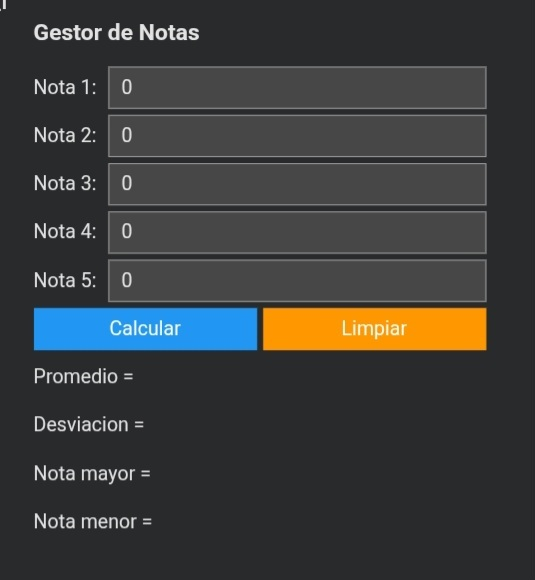
\includegraphics[width=0.55\textwidth]{Screenshot_20261022_083426_Chrome.jpg}
    \caption{Interfaz de usuario simulada para el ejercicio 8.2.}
    \label{fig:ui_82}
\end{figure}

\subsection{Diagramas UML}

\subsubsection{Diagrama de clases}
El diagrama de clases de la figura \ref{fig:clases_82} describe la estructura estática de las clases involucradas en la solución. La clase \texttt{Notas} almacena el arreglo de calificaciones y define los métodos para calcular el promedio, la desviación estándar, la nota mayor y la nota menor. La clase \texttt{VentanaPrincipal} gestiona los componentes visuales de la interfaz gráfica y contiene una instancia de \texttt{Notas}, vinculando los eventos de usuario con las operaciones de cálculo.

\begin{figure}[H]
    \centering
    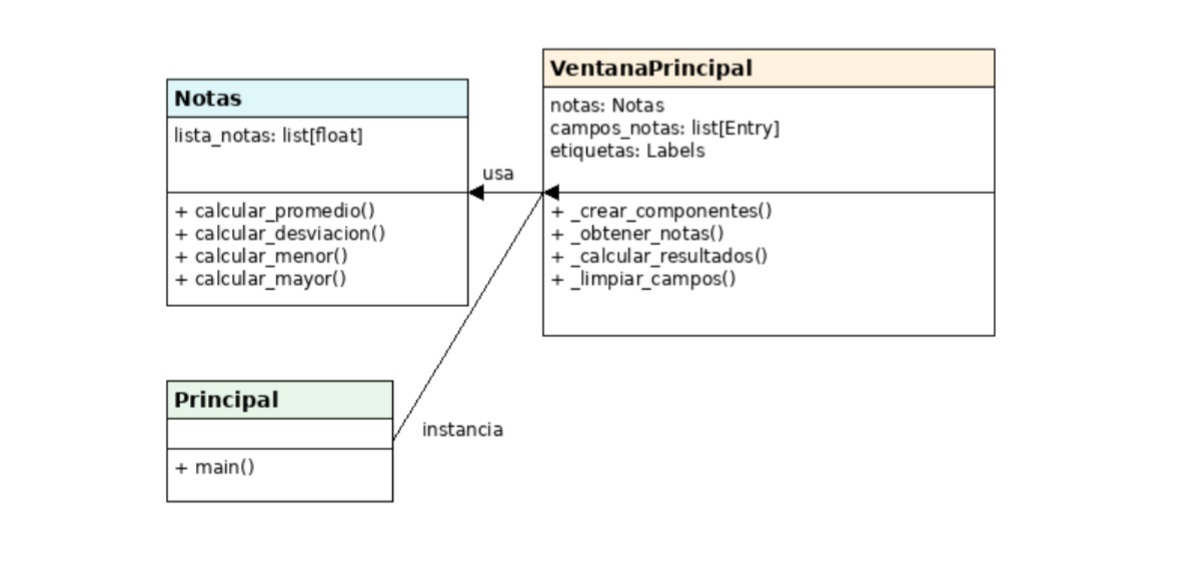
\includegraphics[width=0.85\textwidth]{Screenshot_20261022_110037_Samsung Notes.jpg}
    \caption{Diagrama de clases del ejercicio 8.2.}
    \label{fig:clases_82}
\end{figure}

\subsubsection{Casos de uso}
El diagrama de casos de uso (figura \ref{fig:casos_82}) modela las interacciones principales del usuario con el sistema. El usuario (actor) interactúa con la aplicación mediante las siguientes acciones:

\begin{figure}[H]
    \centering
    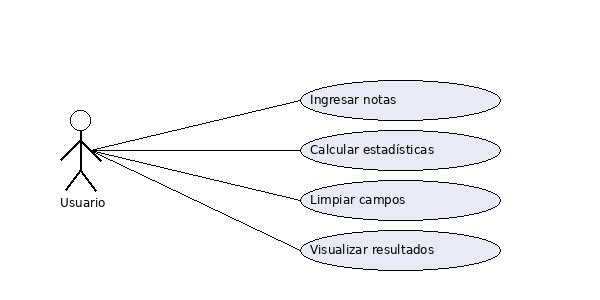
\includegraphics[width=0.85\textwidth]{Screenshot_20261022_110046_Samsung Notes.jpg}
    \caption{Diagrama de casos de uso para el ejercicio 8.2.}
    \label{fig:casos_82}
\end{figure}

\begin{itemize}
    \item \textbf{Ingresar notas:} el usuario introduce cinco valores numéricos correspondientes a las calificaciones.
    \item \textbf{Calcular estadísticas:} al pulsar el botón Calcular, la aplicación valida las entradas, procesa las notas y muestra el promedio, la desviación estándar, la nota mayor y la nota menor.
    \item \textbf{Limpiar campos:} al pulsar el botón Limpiar, se restablecen los campos de entrada y las etiquetas de resultado.
    \item \textbf{Visualizar resultados:} el usuario observa las métricas estadísticas calculadas en el panel inferior.
\end{itemize}

\newpage

% --- SECCIÓN 2: EJERCICIO 8.3 ---
\section{Ejercicio 8.3}

\noindent\textbf{Enlace a GitHub:} \url{https://github.com/yguzmanm-sys/POO-2026-2S/blob/main/Actividad3/Ejercicio8_3.py}

\subsection{Código Fuente}

\begin{lstlisting}[language=Python, caption=Cálculo de volumen y superficie de figuras geométricas, label=lst:ej83]
import math
import tkinter as tk
from tkinter import ttk, messagebox

class FiguraGeometrica:
    """Clase base que almacena el volumen y la superficie de una figura."""
    def __init__(self) -> None:
        self.volumen: float = 0.0
        self.superficie: float = 0.0

    def set_volumen(self, volumen: float) -> None:
        self.volumen = volumen

    def set_superficie(self, superficie: float) -> None:
        self.superficie = superficie

    def get_volumen(self) -> float:
        return self.volumen

    def get_superficie(self) -> float:
        return self.superficie

class Cilindro(FiguraGeometrica):
    """Representa un cilindro definido por su radio y altura."""
    def __init__(self, radio: float, altura: float) -> None:
        super().__init__()
        self.radio = radio
        self.altura = altura
        self.set_volumen(self.calcular_volumen())
        self.set_superficie(self.calcular_superficie())

    def calcular_volumen(self) -> float:
        return math.pi * self.altura * self.radio ** 2

    def calcular_superficie(self) -> float:
        area_lateral = 2 * math.pi * self.radio * self.altura
        area_bases = 2 * math.pi * self.radio ** 2
        return area_lateral + area_bases

class Esfera(FiguraGeometrica):
    """Representa una esfera definida unicamente por su radio."""
    def __init__(self, radio: float) -> None:
        super().__init__()
        self.radio = radio
        self.set_volumen(self.calcular_volumen())
        self.set_superficie(self.calcular_superficie())

    def calcular_volumen(self) -> float:
        return (4.0 / 3.0) * math.pi * self.radio ** 3

    def calcular_superficie(self) -> float:
        return 4.0 * math.pi * self.radio ** 2

class Piramide(FiguraGeometrica):
    """Representa una piramide de base cuadrada con apotema."""
    def __init__(self, base: float, altura: float, apotema: float) -> None:
        super().__init__()
        self.base = base
        self.altura = altura
        self.apotema = apotema
        self.set_volumen(self.calcular_volumen())
        self.set_superficie(self.calcular_superficie())

    def calcular_volumen(self) -> float:
        return (self.base ** 2) * self.altura / 3.0

    def calcular_superficie(self) -> float:
        area_base = self.base ** 2
        area_lados = 2.0 * self.base * self.apotema
        return area_base + area_lados

class FiguraApp:
    FIGURAS = ("Cilindro", "Esfera", "Piramide")
    def __init__(self, root: tk.Tk) -> None:
        self.root = root
        self.root.title("Figuras geometricas")
        self.root.configure(padx=24, pady=24)
        self._construir_interfaz()

    def _construir_interfaz(self) -> None:
        titulo = ttk.Label(self.root, text="Figuras geometricas", font=("Segoe UI", 16, "bold"))
        titulo.grid(row=0, column=0, columnspan=2, sticky="w")
        
        ttk.Label(self.root, text="Seleccione la figura:").grid(row=1, column=0, sticky="w", pady=(12,4))
        self.figura_var = tk.StringVar(value=self.FIGURAS[0])
        self.figura_selector = ttk.Combobox(self.root, textvariable=self.figura_var, values=self.FIGURAS, state="readonly", width=22)
        self.figura_selector.grid(row=1, column=1, sticky="ew", pady=(12,4))
        self.figura_selector.bind("<<ComboboxSelected>>", lambda _: self._actualizar_campos())

        self.campos = {}
        etiquetas = ("Radio (cm):", "Altura (cm):", "Base (cm):", "Apotema (cm):")
        for index, etiqueta in enumerate(etiquetas, start=2):
            ttk.Label(self.root, text=etiqueta).grid(row=index, column=0, sticky="w", pady=3)
            var = tk.StringVar()
            entry = ttk.Entry(self.root, textvariable=var)
            entry.grid(row=index, column=1, sticky="ew", pady=3)
            self.campos[etiqueta] = (var, entry)

        botones_frame = ttk.Frame(self.root)
        botones_frame.grid(row=6, column=0, columnspan=2, pady=(12,8), sticky="w")
        
        self.boton_calcular = tk.Button(botones_frame, text="Calcular", command=self.calcular, bg="#c9d6ff", width=12)
        self.boton_calcular.pack(side="left", padx=(0,8))
        
        self.boton_limpiar = tk.Button(botones_frame, text="Limpiar", command=self.limpiar, bg="#f8caca", width=12)
        self.boton_limpiar.pack(side="left")

        self.resultado_volumen = tk.StringVar(value="Volumen =")
        self.resultado_superficie = tk.StringVar(value="Superficie =")
        
        ttk.Label(self.root, textvariable=self.resultado_volumen, font=("Segoe UI", 11)).grid(row=7, column=0, columnspan=2, sticky="w", pady=(4,4))
        ttk.Label(self.root, textvariable=self.resultado_superficie, font=("Segoe UI", 11)).grid(row=8, column=0, columnspan=2, sticky="w")

        self.root.columnconfigure(1, weight=1)
        self._actualizar_campos()

    def _actualizar_campos(self) -> None:
        figura = self.figura_var.get()
        campos_activos = {
            "Cilindro": ("Radio (cm):", "Altura (cm):"),
            "Esfera": ("Radio (cm):",),
            "Piramide": ("Base (cm):", "Altura (cm):", "Apotema (cm):"),
        }
        for etiqueta, (var, entry) in self.campos.items():
            if etiqueta in campos_activos[figura]:
                entry.configure(state="normal")
            else:
                var.set("")
                entry.configure(state="disabled")

    def _tomar_float(self, etiqueta: str) -> float:
        valor = self.campos[etiqueta][0].get().strip()
        if not valor:
            raise ValueError(f"Ingrese un valor para {etiqueta}")
        return float(valor)

    def calcular(self) -> None:
        figura = self.figura_var.get()
        try:
            if figura == "Cilindro":
                r = self._tomar_float("Radio (cm):")
                h = self._tomar_float("Altura (cm):")
                figura_obj = Cilindro(r, h)
            elif figura == "Esfera":
                r = self._tomar_float("Radio (cm):")
                figura_obj = Esfera(r)
            else:
                b = self._tomar_float("Base (cm):")
                h = self._tomar_float("Altura (cm):")
                a = self._tomar_float("Apotema (cm):")
                figura_obj = Piramide(b, h, a)
        except ValueError as error:
            messagebox.showerror("Datos invalidos", str(error))
            return

        self.resultado_volumen.set(f"Volumen = {figura_obj.get_volumen():.2f} cm^3")
        self.resultado_superficie.set(f"Superficie = {figura_obj.get_superficie():.2f} cm^2")

    def limpiar(self) -> None:
        for var, entry in self.campos.values():
            entry.configure(state="normal")
            var.set("")
        self.resultado_volumen.set("Volumen =")
        self.resultado_superficie.set("Superficie =")
        self._actualizar_campos()

def main() -> None:
    root = tk.Tk()
    FiguraApp(root)
    root.mainloop()

if __name__ == "__main__":
    main()
\end{lstlisting}

\subsection{Interfaz de usuario}
La figura \ref{fig:ui_83} muestra una representación de la interfaz gráfica implementada para el cálculo de figuras geométricas. El usuario selecciona la figura (cilindro, esfera o pirámide) y el formulario habilita únicamente las entradas necesarias para dicha geometría. Los botones realizan el cálculo o limpian los campos, y las etiquetas presentan el volumen y la superficie calculados.

\begin{figure}[H]
    \centering
    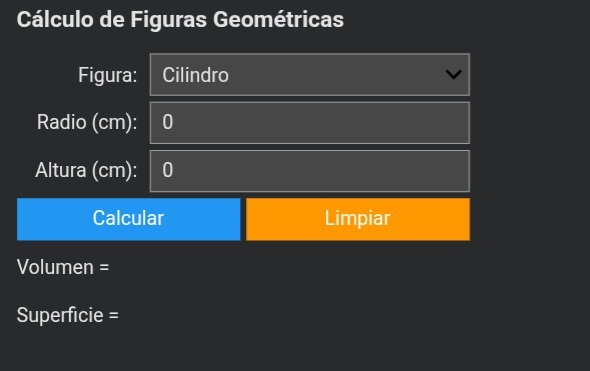
\includegraphics[width=0.55\textwidth]{Screenshot_20261022_083728_Chrome.jpg}
    \caption{Interfaz de usuario para el ejercicio 8.3.}
    \label{fig:ui_83}
\end{figure}

\subsection{Diagramas UML}

\subsubsection{Diagrama de clases}
El diagrama de clases de la figura \ref{fig:clases_83} ilustra la jerarquía y relaciones empleadas en la solución. La clase base \texttt{FiguraGeometrica} encapsula los atributos comunes y define los métodos para fijar y consultar el volumen y la superficie. Las clases \texttt{Cilindro}, \texttt{Esfera} y \texttt{Piramide} heredan de ella e implementan sus propias fórmulas de cálculo.

\begin{figure}[H]
    \centering
    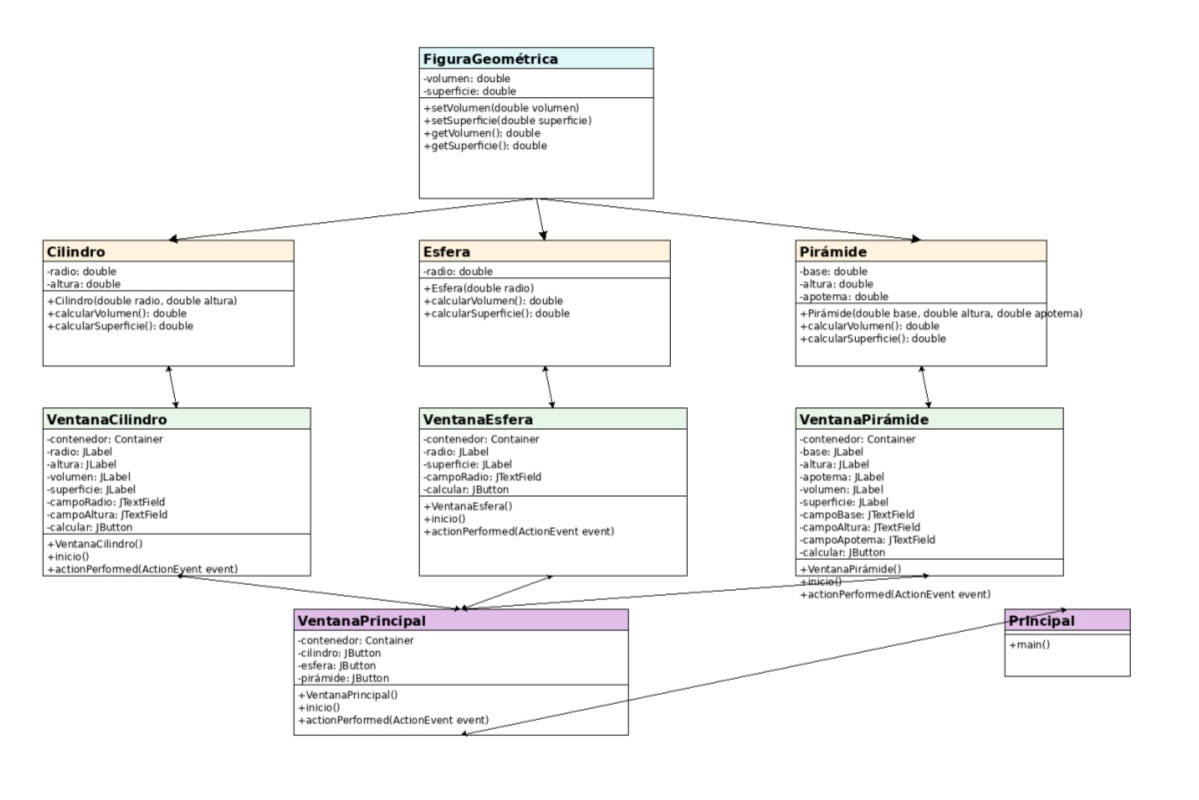
\includegraphics[width=0.85\textwidth]{Screenshot_20261022_110109_Samsung Notes.jpg}
    \caption{Diagrama de clases para el ejercicio 8.3.}
    \label{fig:clases_83}
\end{figure}

\subsubsection{Casos de uso}
En la figura \ref{fig:casos_83} se especifican los casos de uso principales correspondientes a las acciones del usuario en el sistema:

\begin{figure}[H]
    \centering
    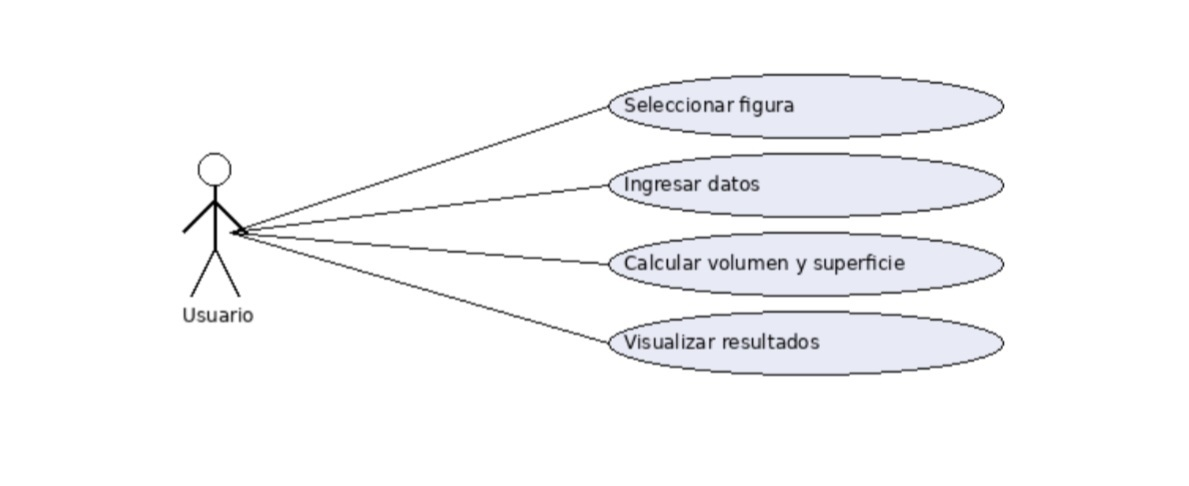
\includegraphics[width=0.85\textwidth]{Screenshot_20261022_110114_Samsung Notes.jpg}
    \caption{Diagrama de casos de uso para el ejercicio 8.3.}
    \label{fig:casos_83}
\end{figure}

\begin{itemize}
    \item \textbf{Seleccionar figura:} el usuario elige la figura geométrica (cilindro, esfera o pirámide) a procesar.
    \item \textbf{Ingresar datos:} se capturan las dimensiones respectivas (radio, altura, base o apotema).
    \item \textbf{Calcular volumen y superficie:} el sistema procesa los valores mediante los métodos de las clases y expone los resultados.
    \item \textbf{Visualizar resultados:} el usuario observa las magnitudes de volumen ($\text{cm}^3$) y superficie ($\text{cm}^2$) obtenidas.
\end{itemize}

\end{document}
